%%%%%%%%%%%%%%%%%%%%%%%%%%%%%%%%%%%%%%%%%%%%%%%%%%%%%%%%%%%%%%%%%%%%%%%%%%%%%%%%%%%%%%%%%%%
%                               My System 24pp
%%%%%%%%%%%%%%%%%%%%%%%%%%%%%%%%%%%%%%%%%%%%%%%%%%%%%%%%%%%%%%%%%%%%%%%%%%%%%%%%%%%%%%%%%%%
\chapter{Prototype}
\label{sec:implementation}

\section*{Summary}
A SleeveAR prototype was built according to our human augmented assistance vision, and complying with the solution requirements.
The prototype had to rely on some already existing devices to implement all planned features, namely for motion tracking and perception and actuation mechanisms for the feedback sources. After describing the system testbed, employed devices, and the setup environment, this chapter will present a description of SleeveAR architecture and its most important implementation details.

\section{Architecture}
\label{sec:impl:arch}

The SleeveAR architecture, which can be seen in Figure~\ref{fig:arch}, relies on several devices for both receiving and sending information.
In terms of input, we are receiving real-time tracking information through an UDP connection with a tracking dedicated computer. Section~\ref{sec:impl:trackdevices} and \ref{prototype-tracking} will explain in more detail what devices were used and how did we actually were able to track a user's arm by using a sleeve with markers.

Given the real-time tracking information, the SleeveAR prototype will then generate user feedback according to a specific exercise the user should attempt to execute. Such feedback was provided by controlling speakers to deliver audio notifications and, most importantly, by making usage of a light projector to project information both on the user's arm and floor. Section~\ref{prototype-projection} explains in detail how this projection was achieved.

\begin{figure}[!t]
    \begin{center}
        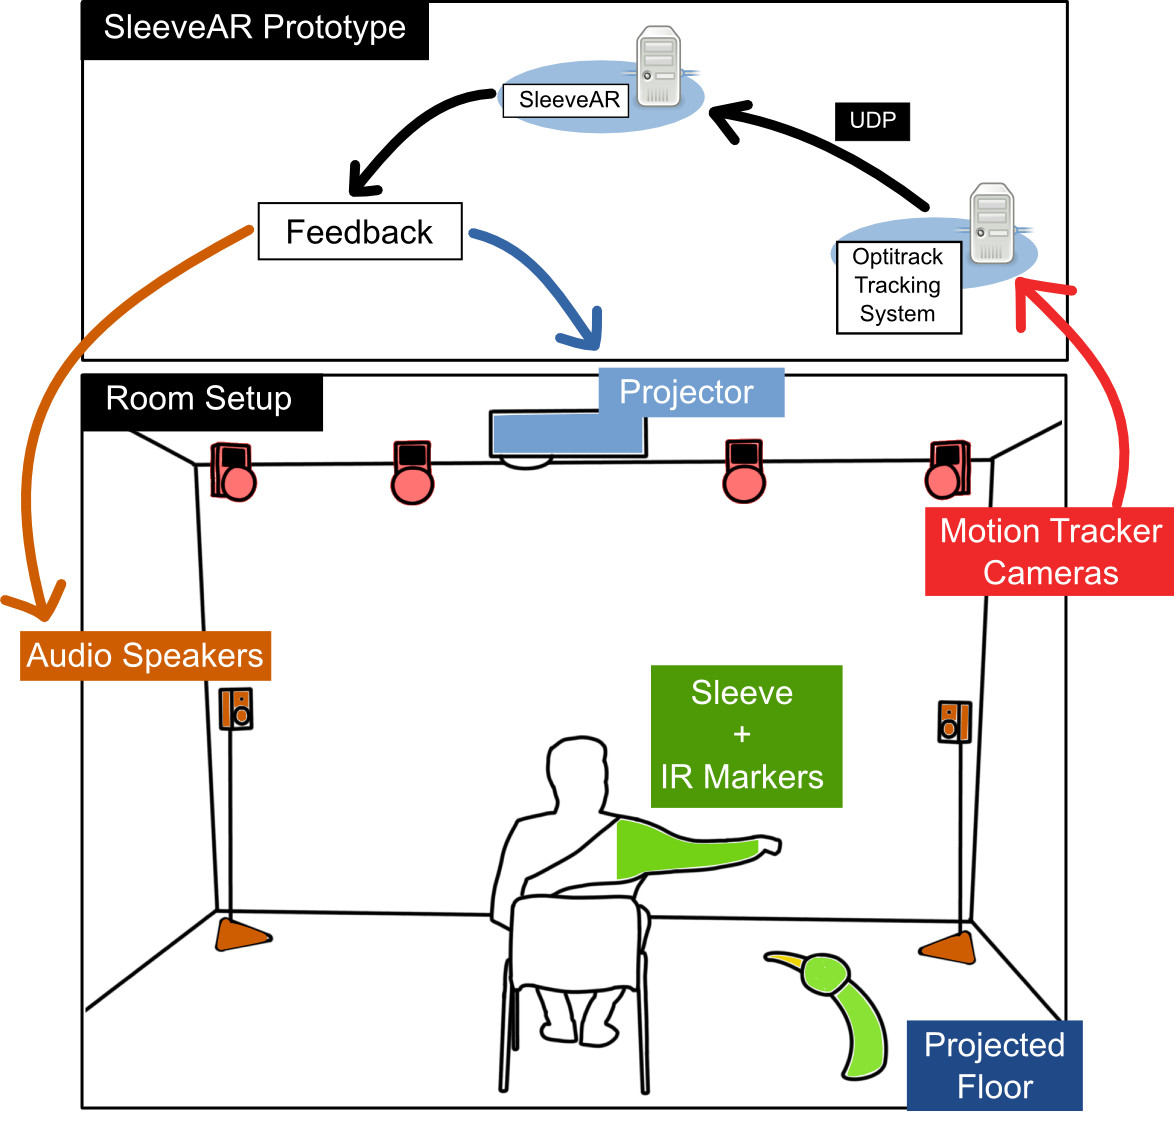
\includegraphics[width=0.7\textwidth]{imgs/impl/arch}
    \end{center}
    \caption{SleeveAR Architecture.}
    \label{fig:arch}
\end{figure}




\section{Tools}
\label{sec:impl:tools}

The SleeveAR implementation was aided with the usage of already existing tools. Tracking devices were employed for capturing and tracking the user movements. Actuator devices, namely audio speakers and video projectors, were also employed as feedback devices to provide corrective instructions for users. The usage of a well known and widely used 3D game engine speeds up the software development process and facilitates interoperability with other systems.

\subsection{Tracking Devices}
\label{sec:impl:trackdevices}

Two different options were considered for choosing the tracking devices.
The first makes use of the recently released, Microsoft Kinect One\footnote{\url{http://www.xbox.com/xboxone/kinect}} 
(previously baptized as Kinect 2), which supposedly offers a better tracking quality than 
the previous version, Kinect 1. Although this might be true, for our implementation we wanted a much more accurate and faster source of tracking. Furthermore, we intended as well to avoid the occurrence of failures due to camera occlusion.

The other available alternative at our laboratories was an OptiTrack Motion Capture system \footnote{\url{https://www.naturalpoint.com/optitrack/}}. 
This option offered us a more precise tracking, and the possibility of dealing with occlusions due to the usage of multiple cameras scattered around the room. 
The downside is the fact that it requires body markers to be carried out by a person for successfully detect him, unlike the 
Kinect, which detects the human body through software algorithms. 

This issue was alleviated by conceiving a comfortable and rather easy way to attach these body markers. A description of how we used the body markers can be found in Section~\ref{prototype-tracking}.


\subsection{Feedback Devices}

Providing effective feedback could be considered one of the foundations of this work. 
We chose to provide both visual and auditory feedback, being the latter much less vital to our goals in this implementation.

As previously described in Section~\ref{sec:sleevear}, our planned visual feedback should be applied on the user's arm and floor. Hence, we relied on a light projector attached to the ceiling of our laboratory to project all visual feedback.
Details about how the light projections were able to hit the correct places, specifically the user's moving arm and floor, will be explained in Section~\ref{prototype-projection}.
Audio feedback was used for simple notifications.
To provide audio, we relied on a speaker system also available at our laboratory.

\subsection{Software}

We chose to implement our prototype with the well known \emph{Unity3D} game engine\footnote{\url{http://www.unity3d.com}}.
This engine already includes several tools that facilitate the development of augmented reality applications. We have in our possession already developed frameworks to communicate with the available tracking devices. In addition, Unity3D uses \texttt{C\#} as its main programming language, which is one of the most common languages use in the game development world, and it already offers a wide range of solutions to create visual information.

\begin{figure}[!t]
\minipage[t]{0.32\textwidth}
  \centering
  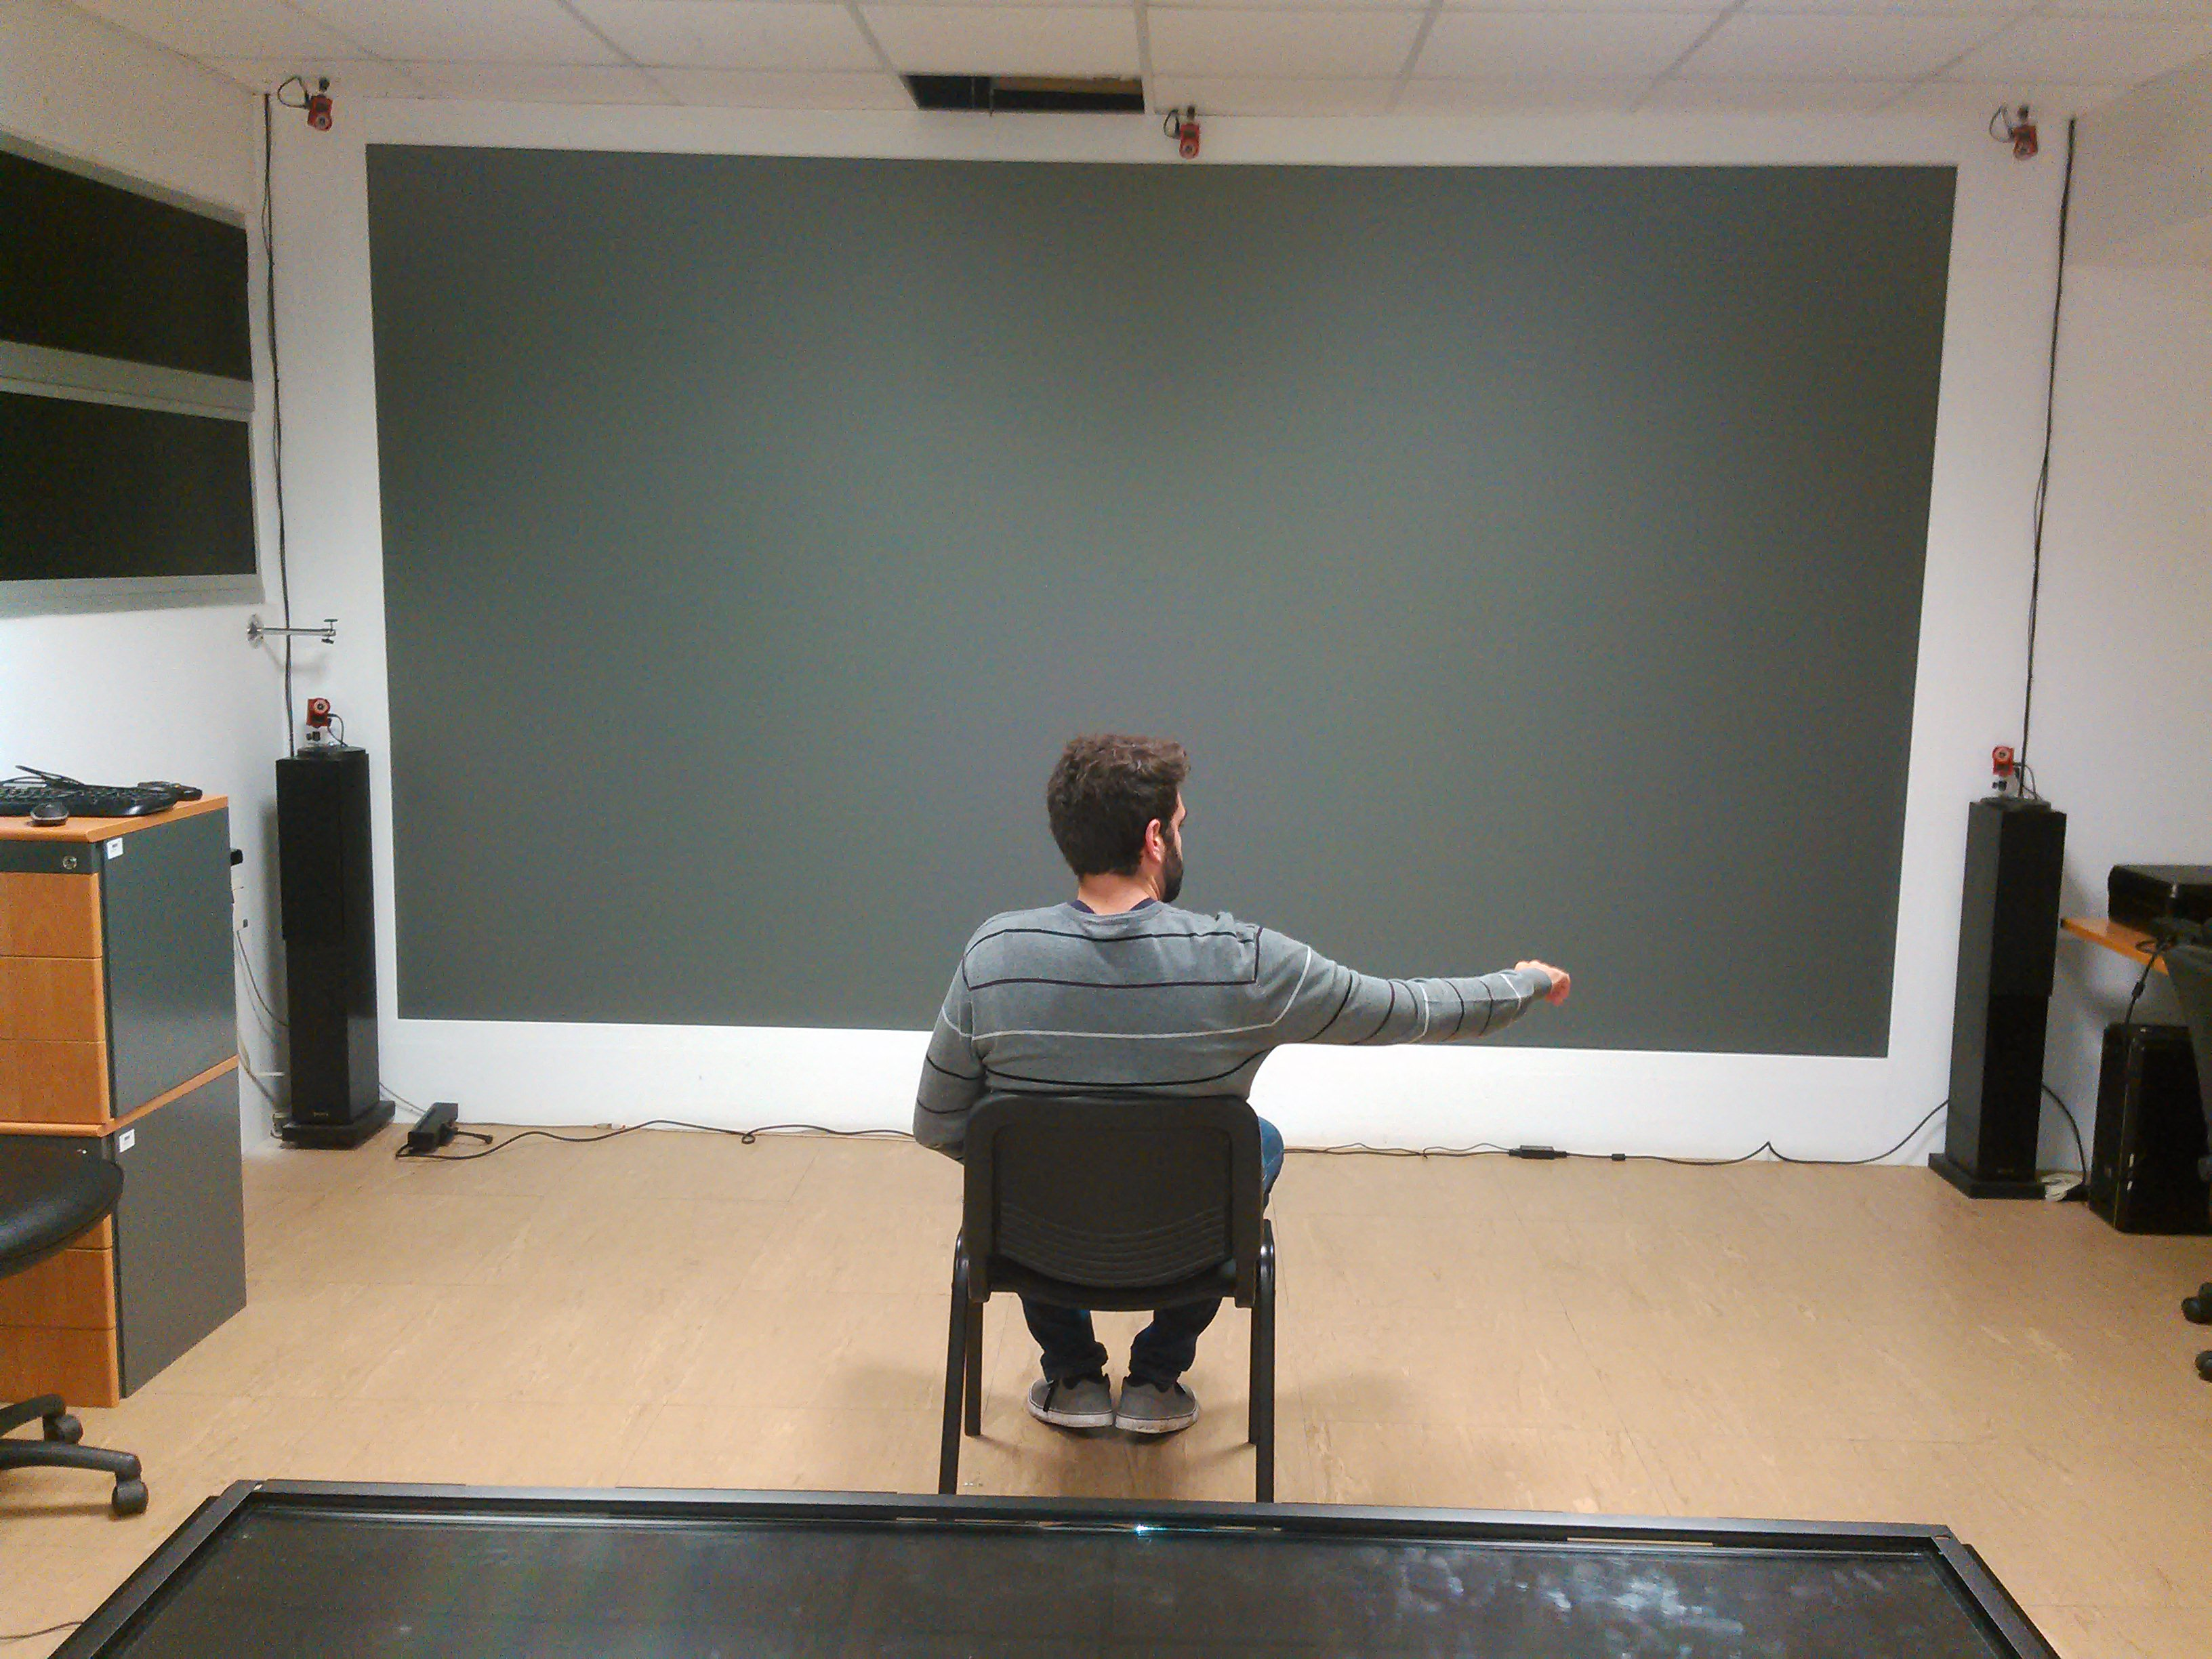
\includegraphics[width=\linewidth]{imgs/impl/laboratory}
    \caption{Work Laboratory.}
    \label{fig:laboratory}
    \endminipage\hfill
\minipage[t]{0.32\textwidth}
  \centering
  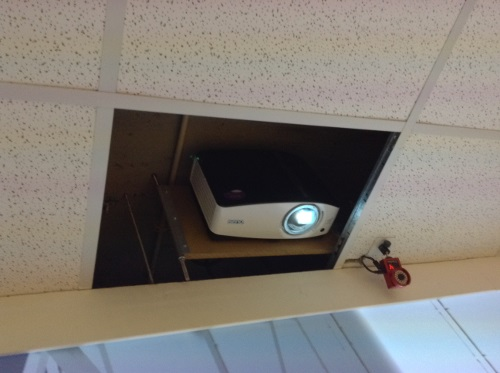
\includegraphics[width=\linewidth]{imgs/impl/projector}
    \caption{Light Projector.}
    \label{fig:projector}
    \endminipage\hfill
\minipage[t]{0.32\textwidth}
  \centering
  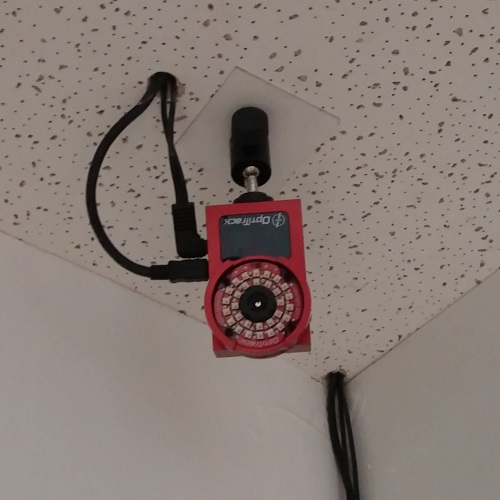
\includegraphics[width=0.75\linewidth]{imgs/impl/optitracksensor}
    \caption{Single Optitrack Camera.}
    \label{fig:optitracksensor}
    \endminipage
\end{figure}

\section{Setup Environment}

All the work here presented was conducted in the Jo\~ao Louren\c{c}o Fernandes Laboratory, located at Campus Taguspark of T\'ecnico Lisboa. This laboratory, shown Figure~\ref{fig:laboratory}, had at our disposal all required devices to implement our work.

There were Optitrack motion sensors already fixed on the walls and prepared to use UDP communication to send tracking data. 
In Section~\ref{prototype-tracking} we will further explain the key points underlying our tracking system.

The light projector is a short-throw Benq MP780 ST+, attached to the ceiling, as seen in Figure~\ref{fig:projector}, and
was connected by a VGA cable to our working computer. We used a resolution of \textit{1280x1024} which resulted in a floor projection of approximately \textit{4.3x3.3} 
meters.

\section{Implementation}

\subsection{Tracking}
\label{prototype-tracking}

\begin{figure}
\minipage[t]{0.32\textwidth}
  \centering
  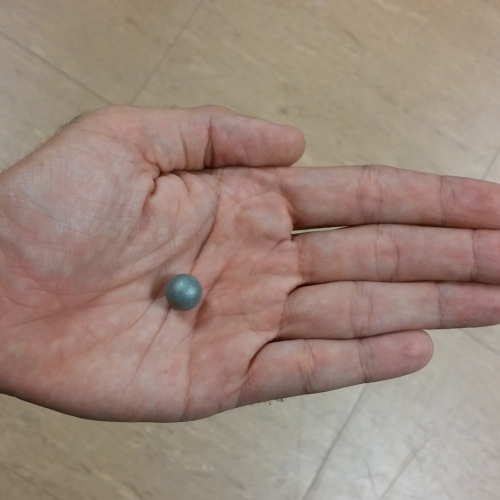
\includegraphics[width=\linewidth]{imgs/impl/singlemarker}
    \caption{Single Tracking Marker.}
    \label{fig:singlemarker}
    \endminipage\hfill
\minipage[t]{0.32\textwidth}
  \centering
  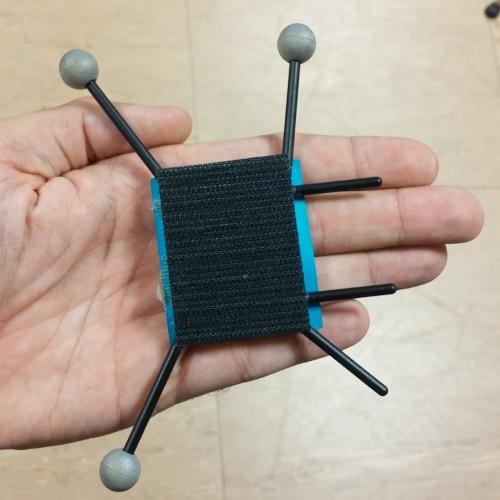
\includegraphics[width=\linewidth]{imgs/impl/markercombination}
    \caption{Marker Combination.}
    \label{fig:markercombination}
    \endminipage\hfill
\minipage[t]{0.32\textwidth}
  \centering
  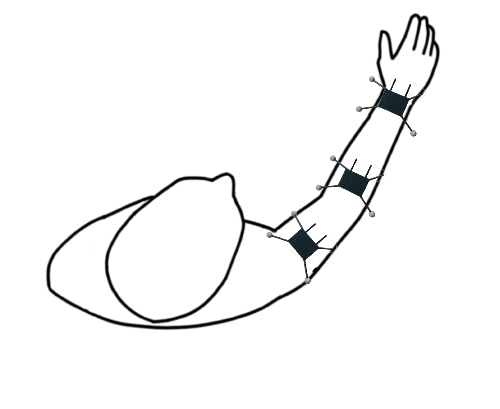
\includegraphics[width=\linewidth]{imgs/impl/rigidbodiesattached}
    \caption{Markers location on arm.}
    \label{fig:rigidbodiesattached}
    \endminipage
\end{figure}


As previously stated, we chose the Optitrack as our tracking system to implement SleeveAR's approach. This tracking system relies on body markers to capture movement.
These body markers are made of reflective material and are usually shaped as small spheres (as shown in Figure~\ref{fig:singlemarker}).
However, Optitrack is not able to track one single marker. Instead, we need to use combinations of markers so that Optitrack calculates both 
position and rotation of the combination's center of mass. 
Small plastic objects were employed to create combinations, onto which was possible to attach several markers exactly as the one being shown in Figure~\ref{fig:markercombination}.

After combining at least three markers, they could be assigned an ID inside Optitrack software. 
From then on, the software was able to identify that specific combination and provide the current position and rotation of the tracked object. Aiming at a simplified writing notation, as well as easier understanding of this thesis, this markers' combination will be hereafter denoted as a \textbf{rigid body}.

As such, three different rigid bodies were required for our solution. Each one should be attached to a different arm location. In this case, shoulder, elbow and wrist. 
With this selection, we were able to receive tracking data from the three locations, and therefore, obtain a virtual model of the arm consisting of these same three locations. In Figure~\ref{fig:rigidbodiesattached} we can observe
an approximate location of each rigid body attached to the arm.

Our first method of placing the each rigid body was by using a Velcro bracelet around each location of the arm. 
Each rigid body would then be attached to each bracelet. This method did not have a positive result for several reasons. 
First, it took to long to attach each bracelet around the arm. In addition, the Velcro material provoked discomfort when pressed hard against the skin. 
Additionally, the bracelets tended to move out of place, especially in the shoulder area where it was particularly hard to properly hold it in place.

Having an easy way to attach, and hard to move, method of holding our rigid bodies was vital for our work. 
Rigid bodies moving out of place during a movement could result in unwanted and unexpected results. 
Therefore, we created a better attachment method, by using a custom designed sleeve.

%\subsubsection{Sleeve}

\begin{figure}[!t]
    \begin{center}
        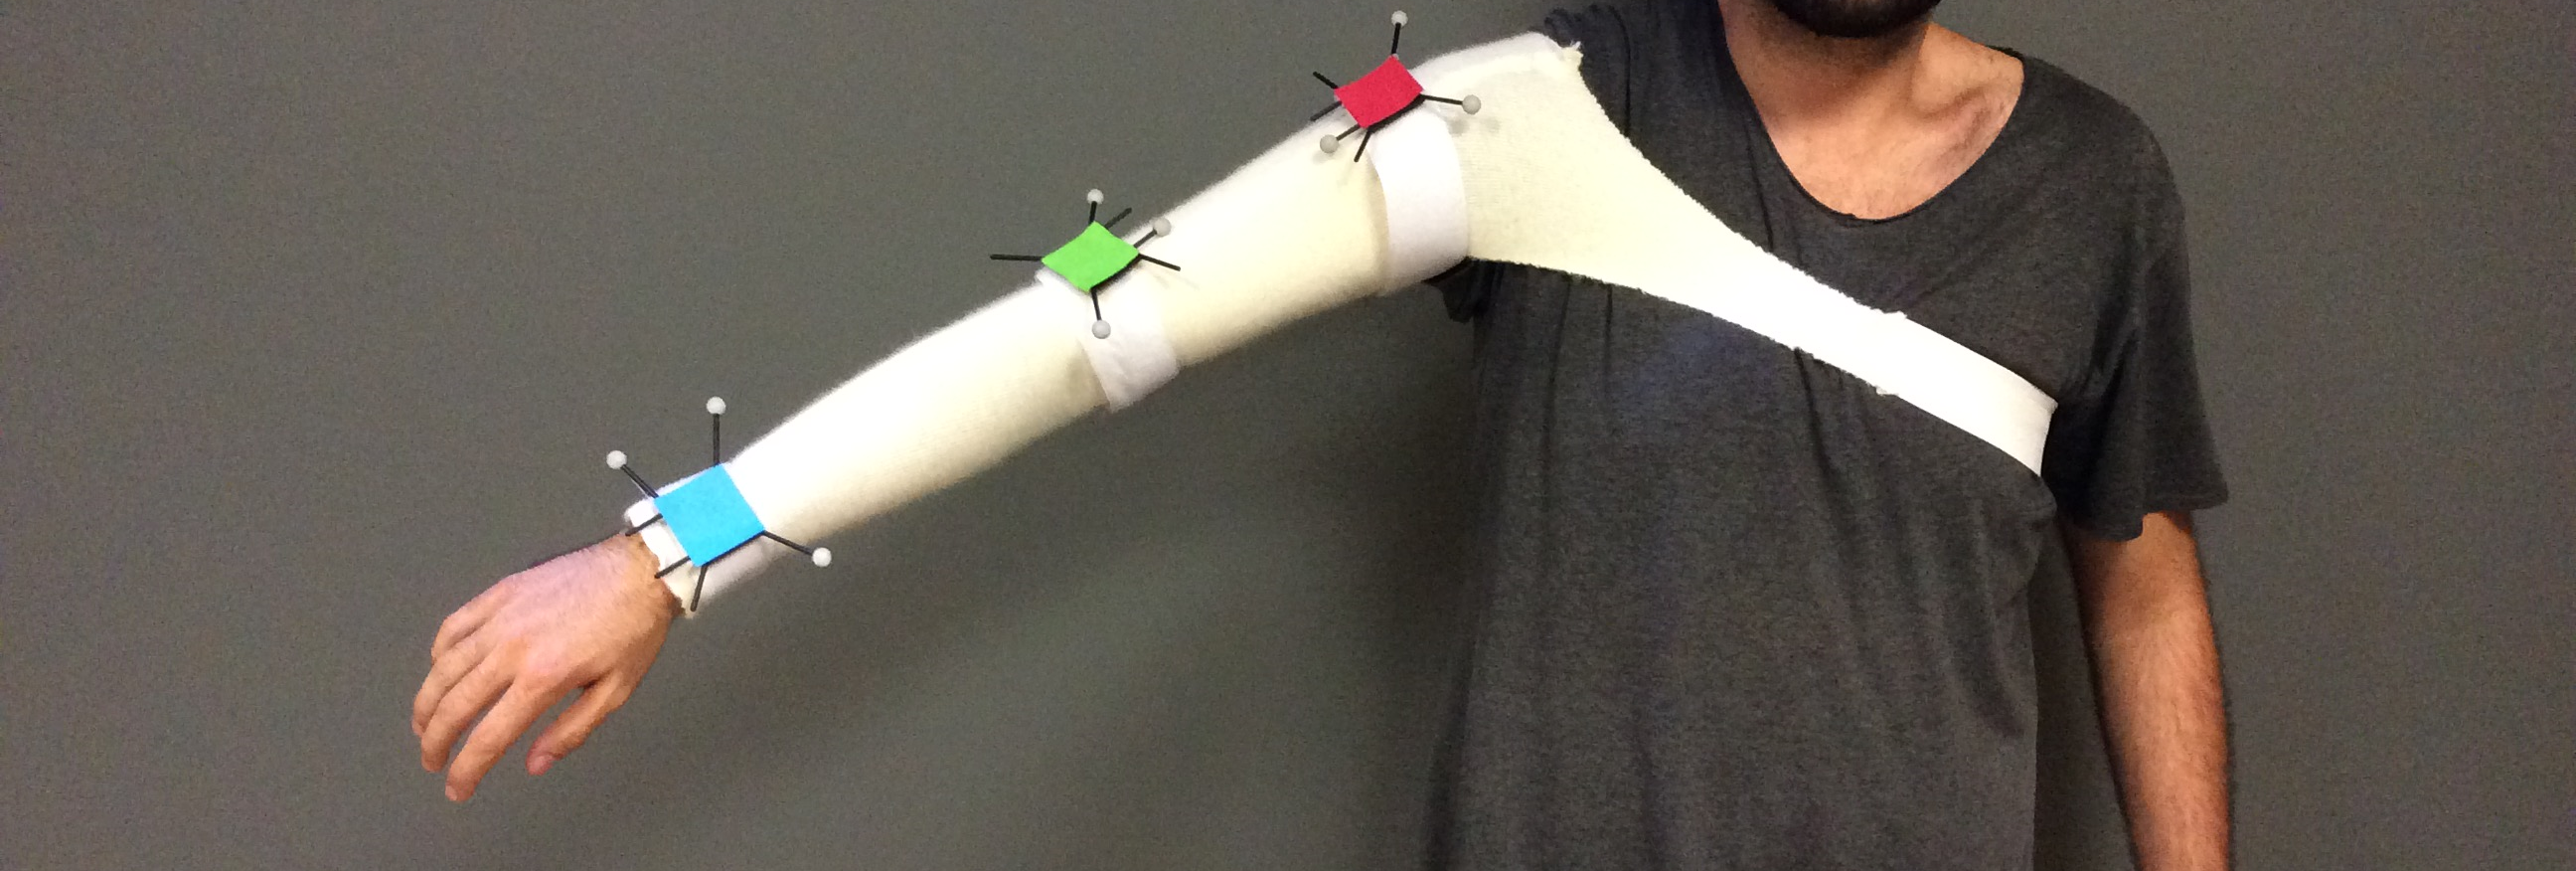
\includegraphics[width=\textwidth]{imgs/impl/sleevewearable}
    \end{center}
    \caption{Sleeve used for tracking.}
    \label{fig:sleevewearable}
\end{figure}

We designed a custom sleeve, as shown in Figure~\ref{fig:sleevewearable}, made out of wool material. 
This solved the above mentioned issues, by fixing the sleeve in place using a kind of "belt" around the user's torso which greatly increased its stability. 
Each of the rigid bodies were still attached to a bracelet, but in this case the bracelets were stitched to the sleeve. 
This improved significantly the rigid bodies attachment due to the bracelets never leaving the sleeve, 
while also enabling us to still squeeze them more or less depending on the user's arm thickness.
Another advantage of using our custom sleeve is providing a better surface to project information, due to its white color. This sleeve enable us to have a smoother and more neutral surface to project information, such as color.  

\subsection{Projection}
\label{prototype-projection}


Projection of visual information in the floor and user's arm was one of the greatest challenges for our implementation. To accomplish it, we divided the implementation into smaller goals.

First of all, we needed to understand the required concepts to project information wherever we wanted. We will use a simple example with a cube being tracked by 
our device, and to facilitate we will use the following nomenclature:

\begin{itemize}
\item \textbf{\ac{PP}} represents the actual position of an object inside the room.
\item \textbf{\ac{VP}} represents the object's 3-dimensional position calculated from the tracking system coordinates
\item \textbf{\ac{PrP}} - 2-dimensional positions on the projected area in the floor.
\end{itemize}




\begin{figure}[!t]
\minipage[t]{0.49\textwidth}
  \centering
  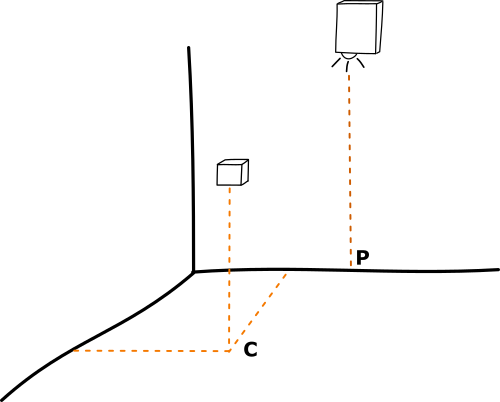
\includegraphics[width=\linewidth]{imgs/impl/projection1}
    \caption{Projection cube example.}
    \label{fig:projection1}
    \endminipage\hfill
\minipage[t]{0.49\textwidth}
  \centering
  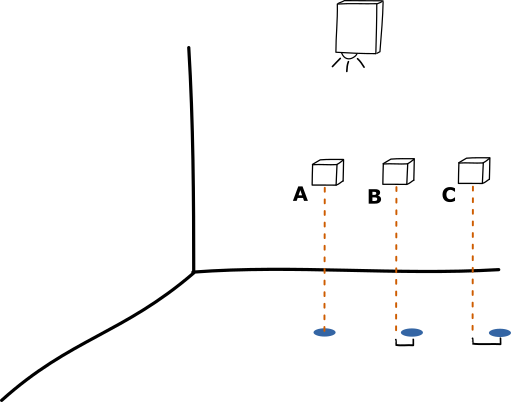
\includegraphics[width=\linewidth]{imgs/impl/projection2}
    \caption{Projected circle offset.}
    \label{fig:projection2}
    \endminipage
\end{figure}



In Figure~\ref{fig:projection1}, a cube inside the room is being tracked by the Optitrack sensor. Hence, we receive its raw positional data, i.e., its \ac{VP}, which is calculated based on the tracking system coordinates' origin.
So, now we know the cube's position in a virtual room. 

If we wanted to project, for instance, a small circle directly below the cube, we would need to find out in which position should the circle be projected (\ac{PrP}) so that it would be below the cube's actual physical position in the room. Hence, we need to find a way of syncing these three different positions, i.e., transforming the different referential, so that the content is easily placed wherever we want. If we tried to simply apply the cube's \ac{VP} position to the projected area, we would encounter several obstacles.

Even though we might have the circle being projected perfectly below Figure~\ref{fig:projection2} A), it was not constantly synced.
If we moved the cube to another \ac{PP}, closer to the edges of the projected area, like in cubes B and C from Figure~\ref{fig:projection2}, the circle would not remain below it. 
Two reasons could cause this. First, the projected area center is not synced with the tracking coordinates center. 
This already generates a small offset in our projection. 
Second, and probably what influences our projection accuracy the most, is the projection distortion closer to the edges.
Looking at Figure~\ref{fig:projection2}, we can see the circle projection getting further away from the desired position if we move the cube between the positions A, B and C.

The first solution to this problem was discovering the correct ratio between what is being tracked what is being projected on the floor. 
If we applied this ratio on our projected content, it could diminish the observed offset. 
Our second solution was to scale the virtual content in order to meet the physical dimensions of the room. 
In other words, looking at Figure~\ref{fig:projection3}, if we projected a line with a virtual length of one unit, the resulting projection on the floor should have a length of approximately one meter.
By doing this, the offsets observed were almost non-existing and even if they were noticeable, we could easily fixed them with some manual offset calibration.

\begin{comment}
\begin{figure}[!t]
    \begin{center}
        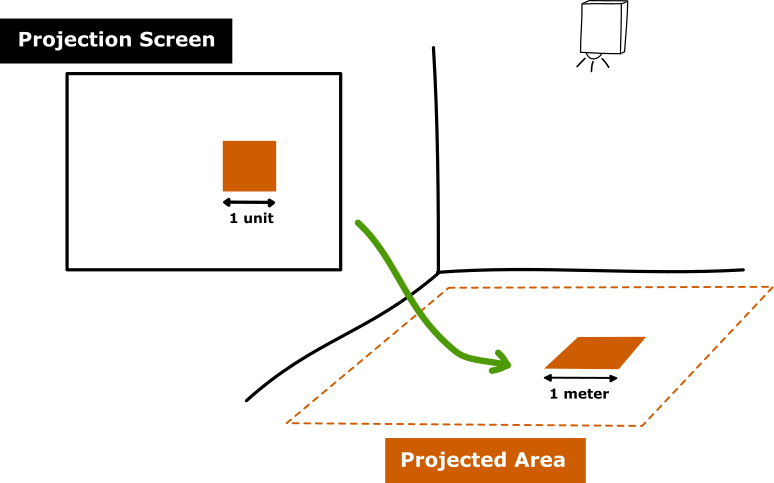
\includegraphics[width=0.5\textwidth]{imgs/impl/projection3}
    \end{center}
    \caption{}
    \label{fig:projection3}
\end{figure}
\end{comment}
After being able to project information directly below any tracked object, our next challenge was to project light on the object itself being tracked. 
In this case, based on our example, we want to project the circle on top of the cube. 
Our challenge here was discovering how a two-dimensional projection could be used to illuminate targets above the floor.

\begin{figure}[!t]
\minipage[t]{0.49\textwidth}
  \centering
  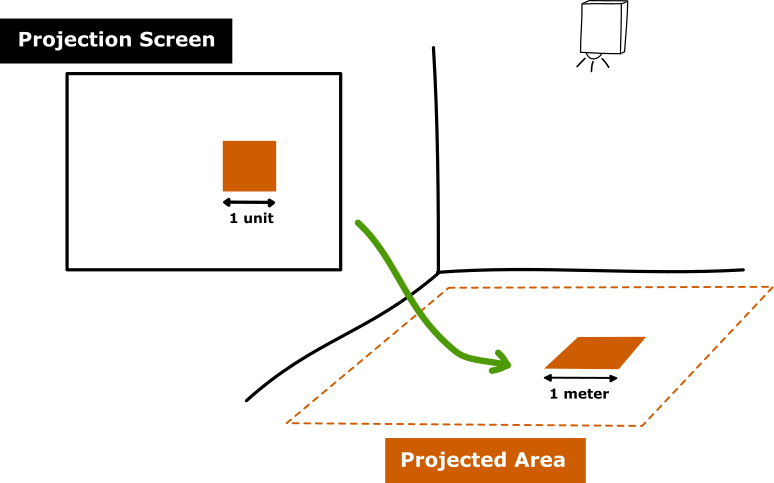
\includegraphics[width=\linewidth]{imgs/impl/projection3}
    \caption{Projected Screen to Projected Area conversion.}
    \label{fig:projection3}
    \endminipage\hfill
\minipage[t]{0.49\textwidth}
  \centering
  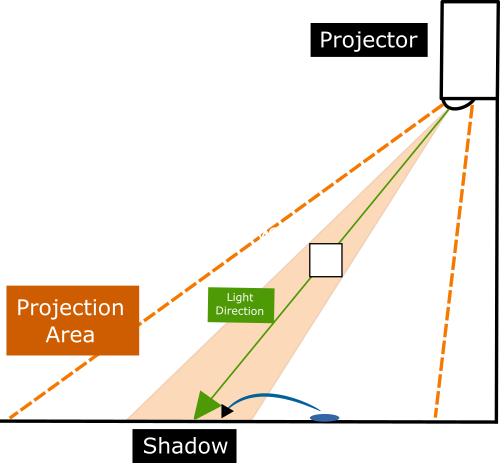
\includegraphics[width=\linewidth]{imgs/impl/projection5}
    \caption{Cube Shadow Side-view.}
    \label{fig:projection5}
    \endminipage
\end{figure}

Looking at Figure~\ref{fig:projection5}, we have a side-view of our example. When the projector light hits the cube, a shadow is created on the floor. 
Since this shadow is still inside the projected area, if we move the circle to its position, it will then be projected on top of the cube.

If we are able to project information where we want (when it comes to floor positions), to hit the cube with light, we need to know the shadow's virtual position. 
To accomplish this, we calculated the projector virtual position and then use it to predict where the shadow would be. 
By simulating the direction a light ray would have when originating from the projector and aimed at a cube, we could achieve a shadow virtual position. 
As is can be seen in fig Figure~\ref{fig:projection5}, by using the \textbf{Light Direction} vector, we reach the shadow virtual position. 
From there we are already able to convert it to the correct physical position. Hence, we are able to hit the actual cube with the circle projection.
When applying this line of thought to our tracked rigid bodies, since there are three rigid bodies attached to our Sleeve, 
we were able to project any kind of content on top of the user's arm.

\subsection{Recording Movements}

\begin{figure}[!b]
    \begin{center}
        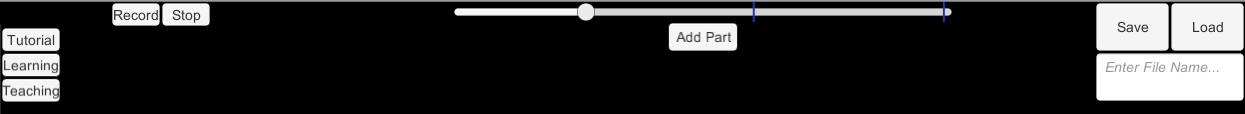
\includegraphics[width=\textwidth]{imgs/impl/recordinginterface}
    \end{center}
    \caption{Recording UI.}
    \label{fig:recordinginterface}
\end{figure}

As previously described in Section~\ref{sec:sleevear:approach}, the prototype should be able to record demonstrated exercises for further use.
We implemented a simple interface to facilitate the recording process.

Assuming the therapist is already wearing the tracking sleeve, the \textbf{record} button, as shown in Figure~\ref{fig:recordinginterface}, simply had to be pressed to enable recording. 
After pressing the recording button, an audio countdown was played through the laboratory speakers, in order to give the therapist some time to place himself at the desired exercise initial position. 
The recording time was set, by default, to a maximum duration of ten seconds, while the rate for capturing the arm tracking data was set to 24 times per second.
The therapist can also stop the recording earlier if the exercise was not intended to take 10 seconds. He simply has to press the stop button.

Immediately after finishing recording, new options appear in the interface. 
A text area can be filled with the intended file name and save the exercise, or first attach more information to the file.

As shown previously in Section~\ref{sec:movementguidance}, visual feedback provided during a movement includes drawing the movement path on the floor. 
But this feedback could become confusing if, for instance, the recorded movement passed twice by the same place. 
The drawn path would intersect with itself, creating an unclear clue to where the movement might go next for the user. 
To avoid this, we implemented the \textbf{exercise parts}, which basically allowed us to divide the exercise in different parts and, consequently, divide also the drawn trajectory generated by the prototype.

To divide an exercise in parts, a slider was available in our interface which, when dragged, allowed to replay back and forth the recorded exercise. 
If the "Add Part" button was pressed, a division would be created in the the exercise based on where the slider currently was positioned.
All of this information was saved along with the exercises and stored on the computer.



\subsection{Data Storage}

The stored files contained a list of all captured data from the three rigid bodies, as described in Section~\ref{prototype-tracking}. 
Each of the list entries contained the position and rotation from each rigid body and also the required information to identify the different exercise parts for assigned exercise parts. Otherwise, the exercises would be treated as one full movement without division.

We chose to save our information in the JSON format, as opposed to XML, because it generates much smaller file sizes. In addition, it is also a more readable format, something useful for the prototype implementation and debugging.

\subsection{Guiding}

Guiding a user through a recorded exercise (the core of this work), involved several phases.

First of all, we needed to load exercise files for them to be used again. 
We decided to use an already existing library, FullSerializer\footnote{\url{https://github.com/jacobdufault/fullserializer}}, for the sole purpose of reading and parsing JSON files.
After loading an exercise file, we could then start guiding a user whenever we wanted.

To implement the planned visual feedback, described in Section~\ref{sec:feedback}, and for it to dynamically change throughout a movement, 
we divided responsibilities into two main components. We will refer to these components as services, more specifically, the \ac{FS} and \ac{ES}.
The \ac{FS} has the responsibility of manipulating the provided feedback while the \ac{ES} was responsible in deciding if the user was executing correctly the exercise.

In other words, it considers an exercise as a list of specific arm directions that the therapist wants another person to replicate in the correct order. 
Obviously, the exercise should start in the first entry of this list. 
Once the user gets close enough to these specific entry, the \ac{ES} will then advance to the next entry. 
This will keep happening until we reach the end of the list and the exercise is over.

With this process in mind, every time \ac{ES} is focused on a specific entry, the information inside it will generate the so called visual feedback \textbf{desired state}. 
Therefore, grabbing the concept of current and desired state from Section~\ref{sec:feedback}, two things will happen. 
First, \ac{FS} will update the current state based on real-time tracking from our current user. 
Second, the desired state will be updated accordingly to the current entry \ac{ES} is focusing on.

Even though we were tracking rigid bodies positions, we could not blindly compare between the original and attempted positions.
As explained in Section~\ref{sec:skeletoncomparison}, the person which recorded an exercise could have, for instance, a different arm length. Hence, even though we were storing rigid bodies positions, we generated normalized vectors to represent the arm direction. 
Upper arm direction was a normalized vector pointing from shoulder to elbow position, while the fore arm direction was a vector from elbow to wrist.
By comparing the directions for both arm regions, we eliminate the physical differences between different user's arm.

\subsection{Performance Review}

Every time an exercise was finished, our prototype should present the user with a review of his attempt. 
As described in our approach, the review should contain trajectory comparison between the original exercise and user's attempt.
As for the score, we implemented a simple formula to return a value from 0 to 100.
Unfortunately, only after finishing our user tests we discovered a better alternative, which we ended up using for our result analysis, in Section~\ref{sec:results}.
A picture of our performance review implementation can be seen in Figure~\ref{fig:teaser} D). \todo{rever este texto...}

\todo{where is described the scoring algorithm ?}


\section{Summary}
